\documentclass{article}

\usepackage[main=english,vietnamese]{babel}
\usepackage[T1]{fontenc}
\usepackage[utf8]{inputenc}
\usepackage[sexy]{evan}
\usepackage{matchsticks}
\usepackage{wrapfig}
\usepackage{listings}

\newtheorem{hint}{Hint}

\title{Proof by Contradiction - Part 2}
\author{Nghia Doan}
\date{\today}

\begin{document}

\maketitle

This article is the second part of the series on demonstration \textit{Proof by Contradiction}.

\begin{example*}[Example 6]
    Twenty-five persons from 8 different provinces elected to the National Congress.
    Prove that at least 4 of them are from the same province.
\end{example*}

\begin{soln}
    Assume that this is not true. Then no $4$ of them are from the same province.
    In this case, not more than $3$ persons are from the $1^{\text{st}}$ province, not more than $3$ from the $2^{\text{nd}}$, and so on.
    Altogether, there are not more than $3 \times 8 = 24$ persons. This contradicts the fact that there are 25 persons.
\end{soln}

\begin{example*}[Example 7]
    At the graduation event of the School of Wizardry, 5 outstanding students called to the podium.
    They standing in a row. Altogether, these 5 students know 300 different spells.
    Prove that there are 2 students standing next to each other who, if combined, know at least 100 spells.
\end{example*}

\begin{soln}
    Suppose that this is not true. Then the $1^{\text{st}}$ and $2^{\text{nd}}$ students together know less than $100$ spells,
    and the $4^{\text{th}}$ and $5^{\text{th}}$ students together know less than 100 spells.
    Then these four know less than 200 spells together. In this case, the $3^{\text{rd}}$ student knows more than $100$ spells.
\end{soln}

\begin{example*}[Example 8]
    The only way to travel in the Kingdom-of-so-many-swamps is to use magic carpets.
    Twenty-one carpet-transportation lines serve the capital.
    A single carpet-transportation line goes to Tinyville,
    and every other city is served by exactly 20 carpet-transportation lines.
    Show that it is possible to travel by magic carpet from the capital to Tinyville
    (perhaps by transferring from one carpet line to another).
\end{example*}

\begin{soln}
    Let's take a look at all the cities that are accessible by magic carpet from Tinyville.
    The capital does not belong to this group. In this group there is a number of cities, each has 20 lines leading to it,
    and one city (Tinyville) with only one line leading to it. Thus the sum of all lines leading to the cities is an odd number.
    But this is not true. If we count the lines among these cities, then they have to be counted twice, thus it is an even number.
    This contradiction means Tinyville is connected to the capital.
\end{soln}

\newpage

\begin{example*}[Example 9]
    The game of Trick-a-Troll is played with 10 players and a deck of 20 cards:
    2 through 10 and an ace of spades, and 2 through 10 and an ace of clubs.
    Each player gets 1 club and 1 spade and adds his cards (aces count as 1).
    Prove that there will be at least 2 players with sums that end in the same digit.
\end{example*}

\begin{soln}
    Let's consider the sum of the values of all the cards.
    If we assume that all players had different last digits for their sums, then all 10 digits would be present, and the sum of them all would end with a 5.
    On the other hand, the sum of the values of all cards in play ends with a 0, a contradiction.
\end{soln}

\begin{example*}[Example 10]
    At each of the vertices of a regular hexagon there stands a grasshopper.
    At the same time, all six grasshoppers jump off the ground. They land at the same time,
    each at one of the vertices. No two grasshoppers land at the same vertex.
    Each of the grasshoppers does not necessarily land at a vertex different from the one it jumps off.
    Prove that there exist three grasshoppers jump off vertices $A, B,$ and $C,$
    and land at $A', B'$ and $C',$ such that $\triangle ABC$ and $\triangle A'B'C'$ are congruent.
\end{example*}

\begin{soln}
    Let assume that it is not possible for such scenario. In other words, if any three grasshoppers jump off vertices $A, B,$ and $C,$
    and land at $A', B'$ and $C',$ then $\triangle ABC$ and $\triangle A'B'C'$ \textit{are not congruent.}

    First, we find out how many types of triangles can be constructed with three vertices of the hexagon.
    There are three types of triangles, such that \textit{they are pair-wise not congruent}, see the diagram below.
    \begin{center}
        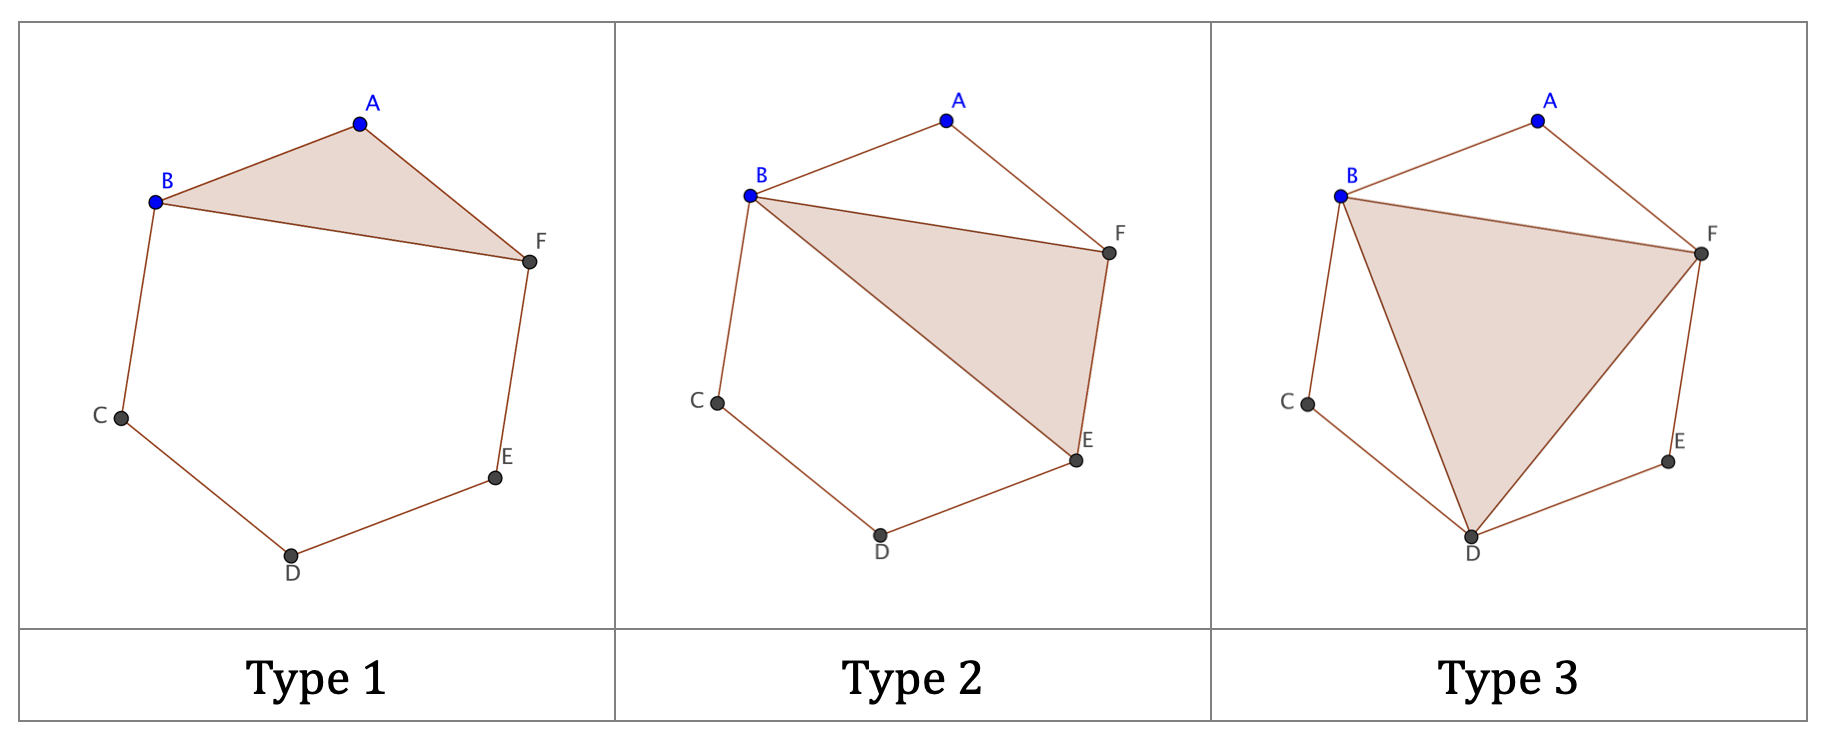
\includegraphics[width=10cm]{./png/sc-23-ms-2-p10.png}
    \end{center}
    
    For \textit{Type 1}, there are 6 such triangles; for \textit{Type 2}, 12 triangles,; and for \textit{Type 3}, 2 triangles.
    (there are 20 such triangles in total.) 

    Now, our assumption means that 12 triangles of Type 2 should be change to the same number of distinct triangles of Type 1 or Type 2,
    which is impossible since there are only $6+2=8$ of them. This is a contradiction.
\end{soln}

\end{document}